\chapter*{Laplace's demon}
\addcontentsline{toc}{chapter}{Laplace's demon}
\begin{center}
\vspace{2cm}
\begin{flushright}
\large
\textit{$\frac{d\mathbf{x}}{dt} = f(\mathbf{x}, t)$ }
\end{flushright}
\vspace{2cm}
\end{center}
\normalsize

\newpage
Pierre-Simon de Laplace conceived a thought experiment involving a hypothetical intelligent being with knowledge of the current state of everything and the capacity to process all that information. Under the hypothesis of a deterministic universe, such a being would know both the past and the future, thereby eliminating the perception of time, since everything that exists now would also reveal what was and what will be.

In a much more limited context of both space and time, the constant monitoring of microscopic changes and patterns places me in a position to predict possible futures and assume causality from potential pasts. I live without a normal perception of time, burdened by the overwhelming anxiety of processing all possible realities with the same intensity as the "here and now." Predicting an experience and experiencing the predictions. Presuming a cause for every effect. 

{\scriptsize \textcolor{comment}{\% Sense belongs to the realm of Aion, not Chronos. }}

Modern physics introduces uncertainty. Quantum mechanics poses that states of matter are probabilistic rather than absolute, breaking the strict determinism of Laplace's vision and the classical Newtonian perspective. Yet, even in a probabilistic universe, the human experience of time remains a construction rather than a fundamental entity.

Deleuze, in \textit{"The Logic of Sense"}, contrasts two modes of time: Chronos, the linear, measurable time of physics, and Aion, the time of pure becoming, where past and future exist in a non-hierarchical relationship.\citep{deleuze1969}

In the context of the digital arts, the idea of predictability often manifests itself in a form that simulates control while embedding elements of randomness and chaos, allowing the viewer to experience the tension between determinism and uncertainty. Generative artworks often operate through algorithms to create an aesthetic of deterministic emergence, where each iteration is governed by pre-defined rules yet appears unpredictable to the observer. A perfect example could be the Conway's \textit{"Game of Life"} \citep{wiki:gol}.\footnote{The Game of Life is a cellular automaton created by John Horton Conway in 1970. The evolution of the game is determined only by its initial state, requiring no further input.}

%% image
\begin{figure}
    \centering
    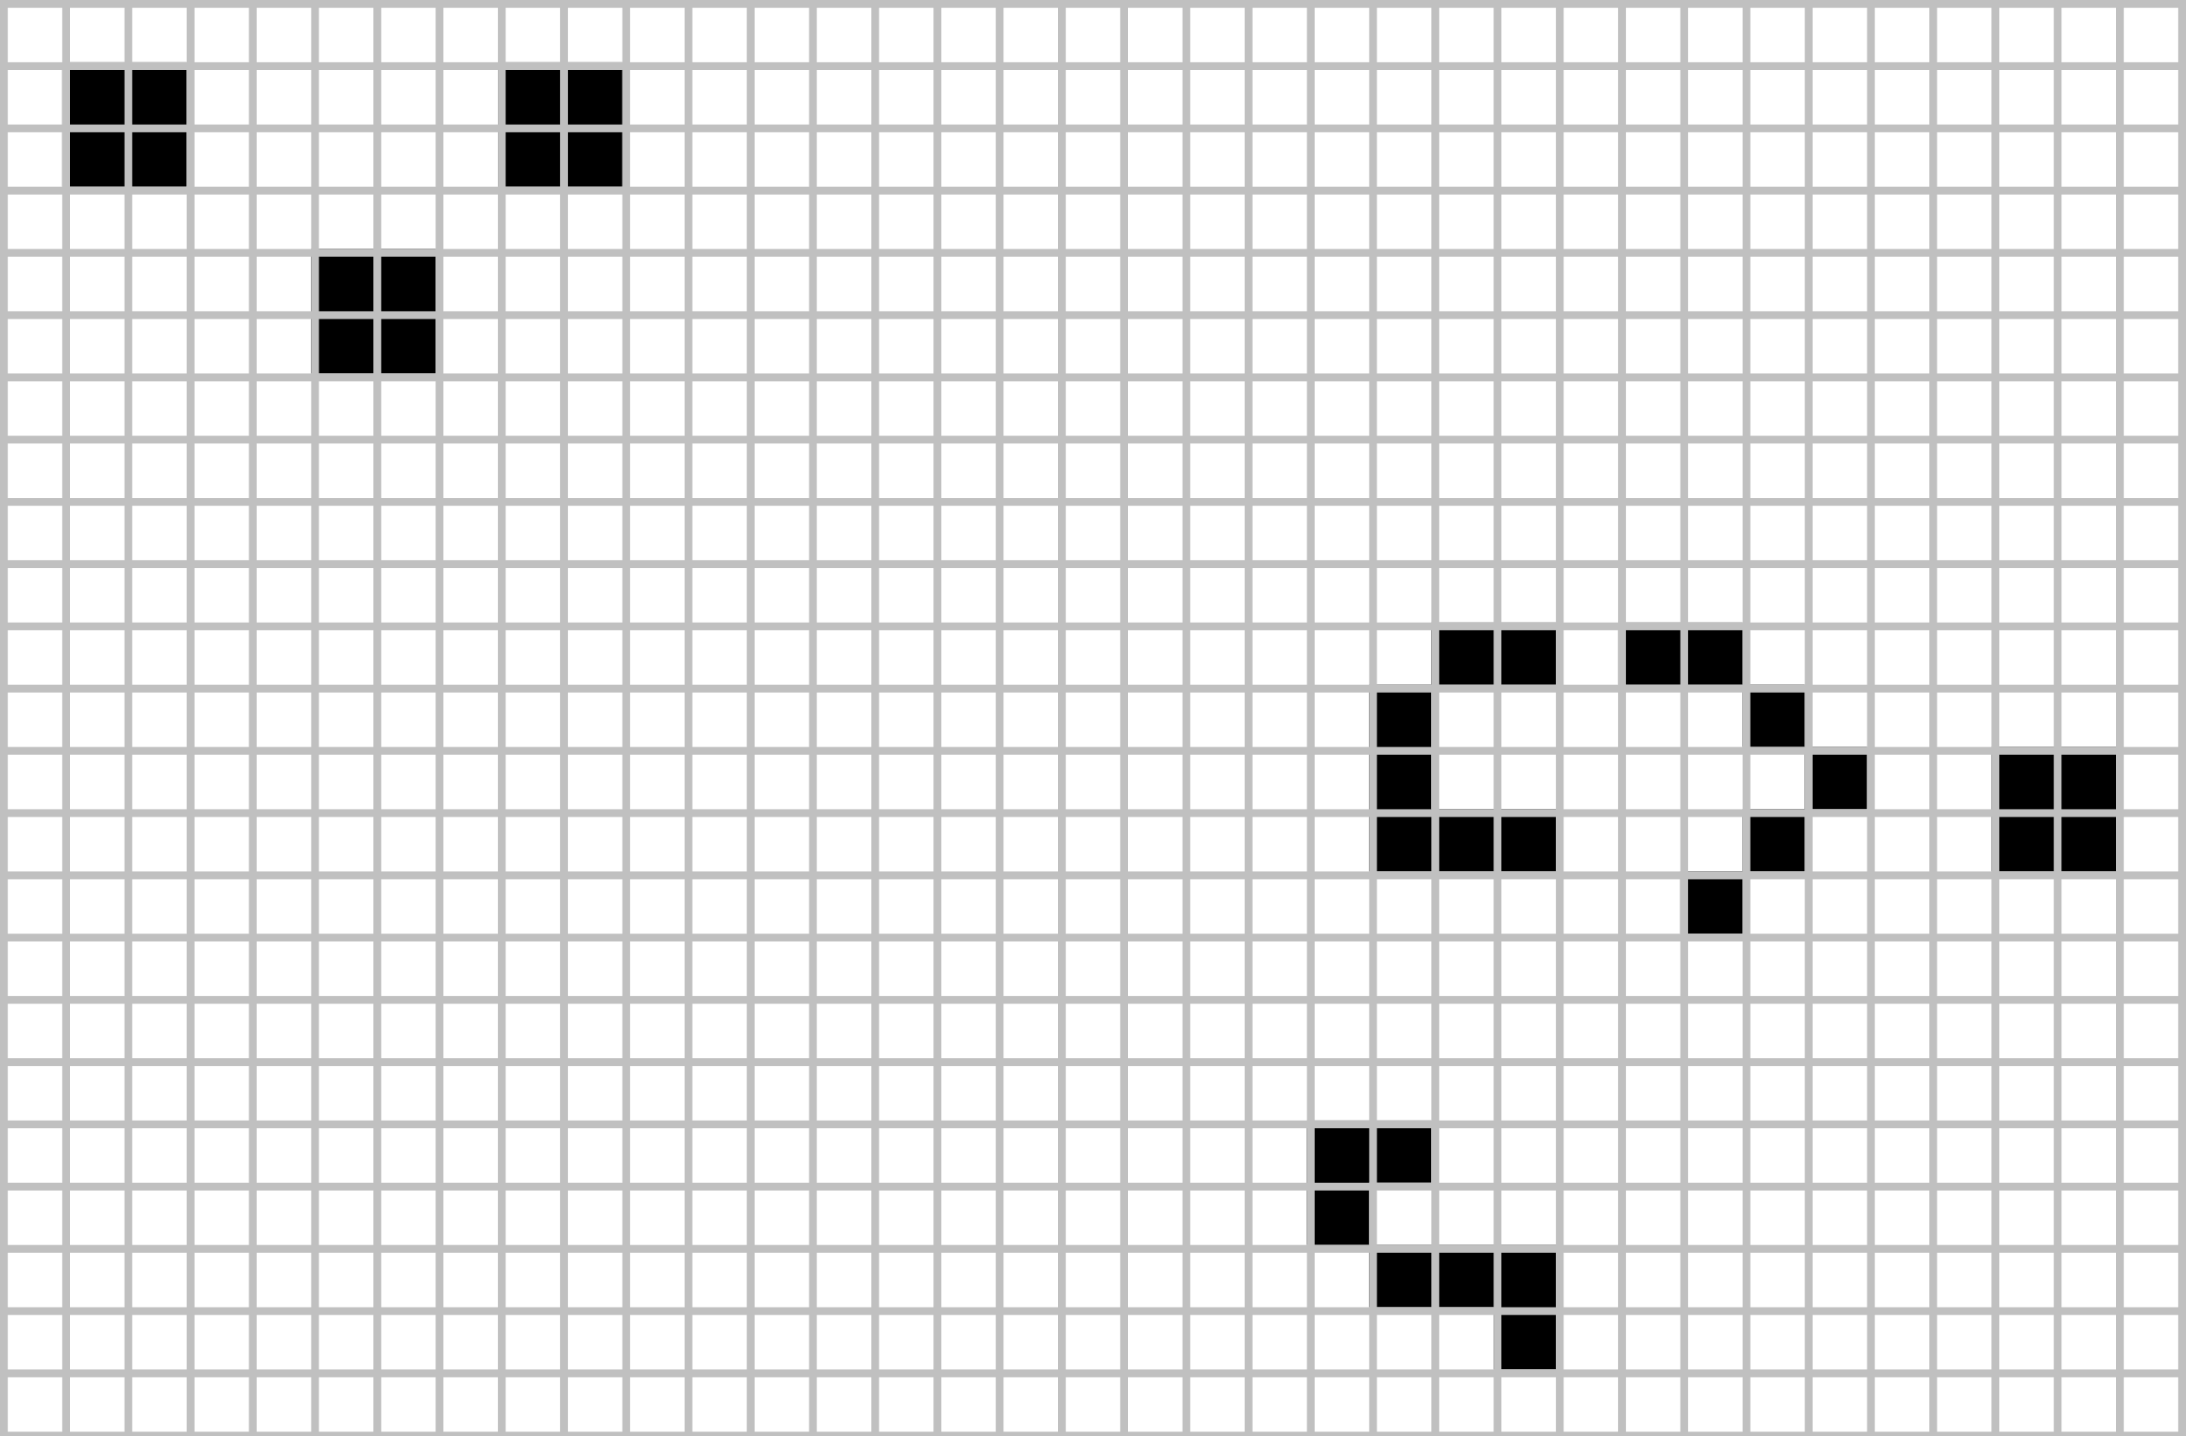
\includegraphics[width=0.8\linewidth]{assets/gol.png} 
    \caption{\small Simkin glider gun - \textit{Conway's Game of Life}.}
    \label{fig:gol}
\end{figure}

Machine learning models, trained on vast amounts of data, function as modern-day deterministic oracles, forecasting human behavior, market fluctuations, and even criminal activity. These systems, however, are not infallible, as they rely on probabilistic statistics rather than absolute determinism. Nonetheless, they shape perception, creating a feedback loop where past behavior is used to constrain future choices.

Social media algorithms, for example, predict and curate content based on prior interactions, effectively scripting a deterministic version of personal experience. The more data fed into these systems, the more precise their predictions, reinforcing a perceived loss of agency. In this context, Laplace's Demon is not an abstract philosophical construct but an active, operational force in digital culture.

If absolute determinism were possible, all uncertainty would dissolve into a singular, knowable timeline. But in reality, the human experience remains shaped by probabilities, contingencies, and incomplete information. This paradox between the desire for predictability and the impossibility of absolute foresight can create a psychological state of hypervigilance.

% Hypervigilance is a cognitive condition characterized by heightened awareness, an intense sensitivity to patterns, and a near-constant anticipation of future events. It is an adaptation to perceived threats, yet in an environment saturated with predictive models and algorithmic forecasting, hypervigilance becomes chronic rather than situational. The act of perpetually calculating possible futures mirrors Laplace’s Demon on a smaller scale: every interaction, every decision, is evaluated through countless imagined trajectories, leading to anxiety rather than clarity.
% % 
The french philosopher Jean-François Lyotard, in his critique of metanarratives, argues that grand deterministic structures burden individuals by imposing rigid explanations onto an inherently chaotic reality \citep{lyotard1979}. The belief that past data can fully determine future events echoes the totalizing narratives of modernity, which attempt to rationalize history through economic, political, or technological inevitabilities. In the digital age, this deterministic burden manifests through algorithmic governance. 

The ubiquitous predictive systems often produce a constructed perception of certainty rather than actual knowledge. The individual caught in this deterministic loop faces a double bind: an overwhelming sense of inevitability (that the future is already decided) paired with the responsibility of optimizing every choice within that rigid structure. This, in turn, reinforces hypervigilance, where every action is analyzed not just in the present but across all its potential future iterations.

% 
The psychological toll of living under predictive determinism can be likened to a mental simulation overload.
We are naturally inclined toward predictive processing, constantly modeling future possibilities based on prior experience and current states. In an age dominated by real-time data analytics, this cognitive mechanism is stretched beyond its evolutionary purpose, forcing us to process an exponential number of possibilities at once. This inevitably creates an experiential paradox, since increase knowledge doesn't always result in greater agency. Anticipating all possible futures does not necessarily provide control, only more paths for anxiety.
% 

%
Time-based media, such as performance art and interactive installations, challenge determinism by requiring live, unrepeatable participation. These works cannot be fully anticipated or reconstructed, embodying contingency and resisting Laplace's hypothetical absolute knowledge. To resist the determinism imposed by both philosophical constructs and algorithmic systems, art and media practice must continue to foreground unpredictability, contingency, and the indeterminacy of human experience.

%   note: examples ? 
%  Lygia Clark – Developed relational objects that require audience manipulation, resisting predefined artistic outcomes.
% Marina Abramović – Uses audience participation in performances to explore contingency and endurance (The Artist is Present).
The artist Ryoji Ikeda famously incorporate randomness in real-time audiovisual installations. Allowing participation and interactivity in the pieces presents a way to discourage determinism. The sound piece titled \textit{"A [for 100 Cars]"} is a good example of it. For this performance, Ikeda invited 100 drivers to follow a score using their cars. Each car was equipped with a sine wave synthesiser producing the note "A" ( frequencies ranging from 376.3 to 506.9 Hz)\footnote{Frequencies ranged from 376.3 to 506.9 Hz represent different historical conventions for the concert pitch, covering a timespan from 1361 to 1936.}, connected to the sound system. The score instructed the drivers to set the octave and volume of the sinewave and to use of lights and horns, or open and close the car doors. The only controlled element is a digital timer and the score sheet provided to every driver. The piece is then conditioned by human action, imperfection and error, making it unique and unpredictable. 

Our experience depends on the flow of time, on uncertainty, on the interplay between memory and expectation. Media, art, and technology constantly negotiate between determinism and randomness, constructing and deconstructing the perception of temporal order.


% {\scriptsize \textcolor{comment}{\%  science fiction}}

